\chapter{Machine vision}

\Gls{machinevision} is the branch of \Gls{ai} focussed on image processing.
The machine vision task performed in this work is called instance \Gls{segmentation}.
In this chapter, I explain what this means. 
The task of segmentation is compared to other machine vision tasks.

This work investigates the used of \Gls{weaklysupervisedl} data for training an Instance segmentation model. 
The concept and benefits of \Gls{weaklysupervisedl} machine learning are explained.

\section{Machine vision tasks \label{sec:machinevisiontasks}}

\Gls{machinevision} is a broad discipline. 
Humans extract information from images almost subconsciously and we are often not aware of the different tasks we perform on images.
The objective of this section is to briefly define different machine vision tasks discussed further in this book. 


Several machine vision tasks consist of \textit{recognizing} objects, animals or humans in an image.
A model is build for a finite list of \textit{categories} that can be present in an image.
Depending on the question asked ad inference time, on can distinquish the following tasks.

\begin{description}
    \item[Image classification] is the task of determining what object category\footnote{or categories} is present in the image. Is there a cat in this image?
    \item[Object counting] is the task of counting how many instances of each category can be seen in the image. How many cats are there in this picture? 
    \item[Object detection] consists not only of identification of the object. Also the spatial position is requested. This is often requested in the form of a bounding box. Where is the cat in this picture, if a cat is present?
    \item[Semantic segmentation] requires that for each image pixel, a class is estimated. Pixels that do not belong to a specific class are called the \textit{background}.
    \item[Instance segmentation] requires not only that the semantic class is determined for each pixel, but also that two individuals of the same class\footnote{say, two cats.} are distinguished.   
\end{description}

The difference between these machine vision tasks is illustrated in figure \ref{fig:machinevisiontasks}. 

\begin{SCfigure}[][h!]
    \centering
    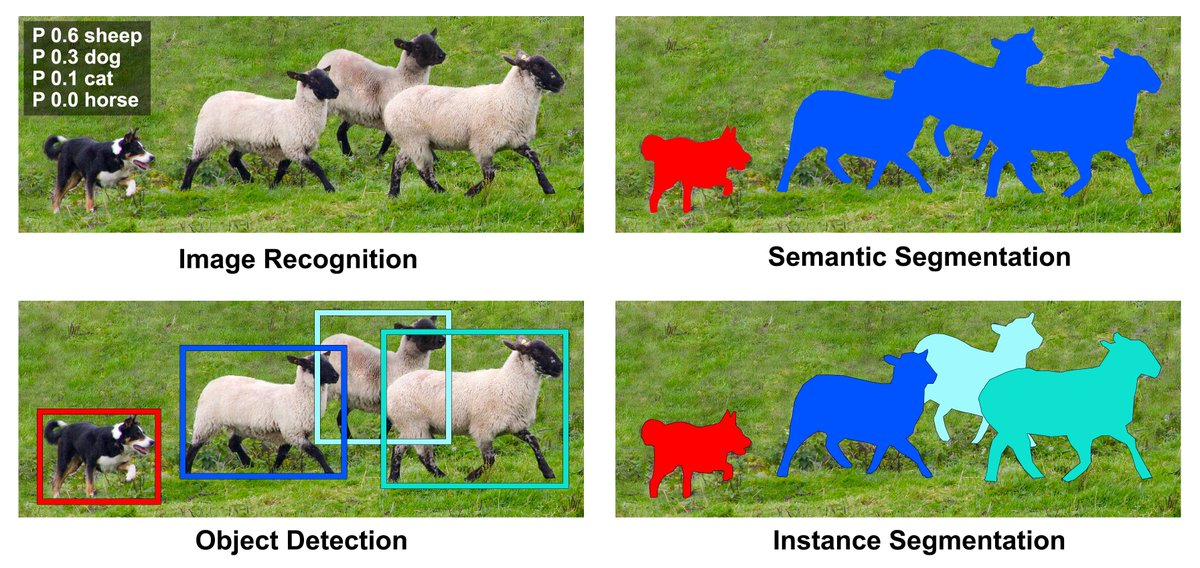
\includegraphics[width=10cm]{/home/thesis/images/Classification_vs_Segmentation.jpg}
    \caption{Illustration to compare different Machine vision tasks \cite{SemTorch76:online}. 
    Object detection means that the location of several objects is estimated by the model. This is indicated by the \textit{bounding boxes}.
    Segmentation of an image is the process of classifying each pixel in the correct class or assign it to the \textit{background} class.
    Semantic segmentation makes no difference between different instances of the same semantic class, instance segmentation does.
    \label{fig:machinevisiontasks}}
\end{SCfigure}

Other interesting applications of \gls{machinevision} include\footnote{This list is not exhaustive.}:
\begin{description}
    \item[Face recognition] is the identification of human faces. 
    \item[Image reconstruction] or \textit{inpainting} consists of recreating parts of a damaged image.
    \item[Image captioning] consists of the creation of full sentences describing the content of an image.    
\end{description}

\section{Supervision types}

To build a model to perform the tasks discussed in \ref{sec:machinevisiontasks}, this model needs to be trained.
This requires a set of \textit{labelled} images. 
This means that a collection of images needs to be provided where an expert in the intended task has provided correct information the model can \textit{learn} from.

Depending on the model objective, other types of labelling are required.

\begin{SCfigure}[][htb]
    \centering
    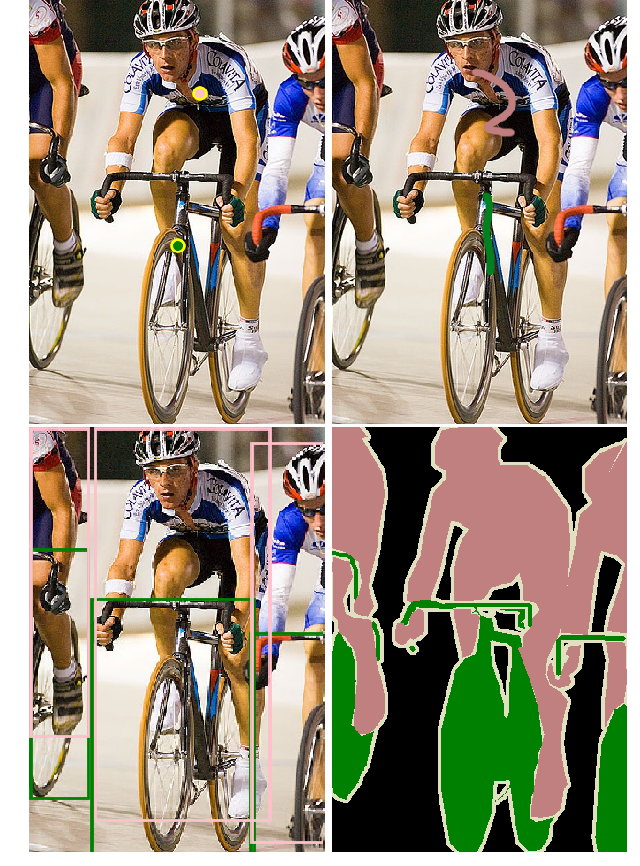
\includegraphics[width=10cm]{/home/thesis/images/McEver.png}
    \caption{Four different annotation types \cite{McEver2020}: 
    On the top left the picture is point level annotated. The points are inflated for visibility.
    On the top right, squiggle annotation is used.
    The bottom left shows bounding box supervion.
    While the bottom right image is fully annotated.
    An image level label would indicate that there are multiple instances of \textit{person} and \textit{bike} in the image.
    }
\end{SCfigure}

The generation of these labels is very expensive and time-consuming.
Especially \gls{deepl} models are known to be very data-hungry. 
These models have determined unprecedented performance, provided sufficient data has been provided.

\todo[inline]{Motivation of weakly supervised learning --> Difference in annotation time and cost from Bearman and Laradji Covid}